\subsection{Gantt Chart}

The Gantt chart maps the eight-sprint schedule against a calendar timeline, showing which modules are built in which weeks and where activities overlap \cite{gantt1}. Each sprint occupies a four-week block. The chart makes it easy to see, at a glance, whether requirements work is closing before implementation begins, and whether testing starts early enough to catch integration failures before the final sprint. Figure~\ref{fig:ganttchart} shows the full timeline.

\begin{figure}[H]
\centering
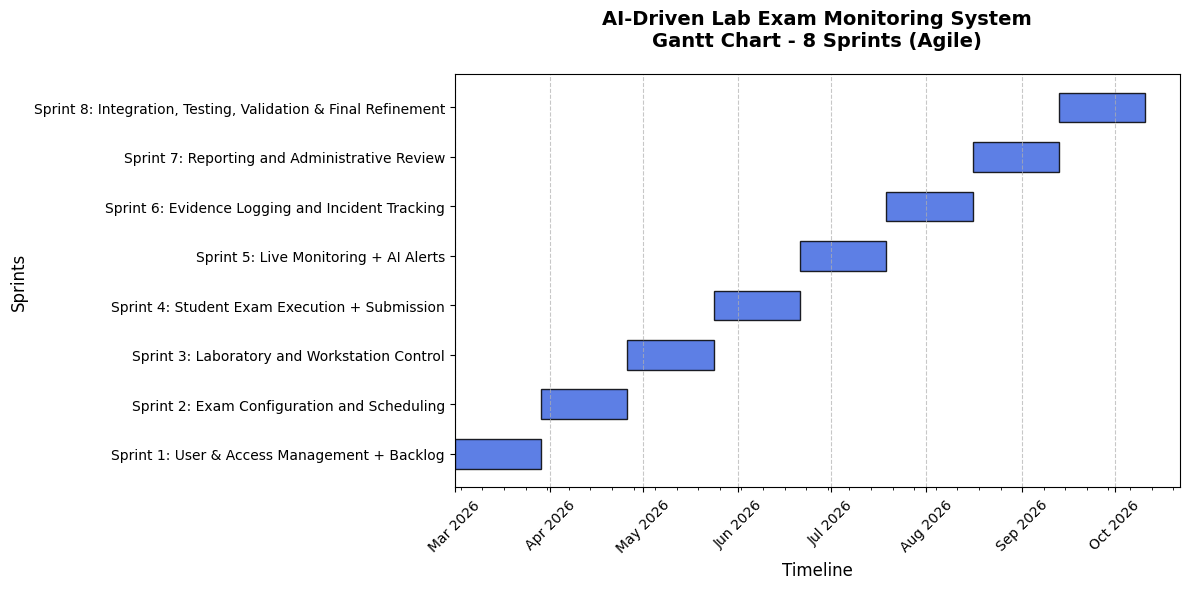
\includegraphics[width=0.95\linewidth]{Figures/gantt_chart.png}
\caption{Project Gantt Chart Based on Eight Agile Sprints}
\label{fig:ganttchart}
\end{figure}

The chart in Figure~\ref{fig:ganttchart} must be read alongside the sprint descriptions in Chapter 1.8. Each bar represents work within a sprint increment, not a waterfall phase. If a sprint review reveals that a module is not ready, the Gantt chart is updated before the next sprint begins \cite{spp1}.

\subsection{Work Breakdown Structure}

The Work Breakdown Structure (WBS) decomposes the project into individual work packages \cite{wbs1}. At the top level, the project splits into five major areas: Requirements, Design, Implementation, Testing, and Documentation. Implementation then breaks further into the twelve module clusters defined in the product scope. Figure~\ref{fig:wbs} shows the full decomposition.

\begin{figure}[H]
\centering
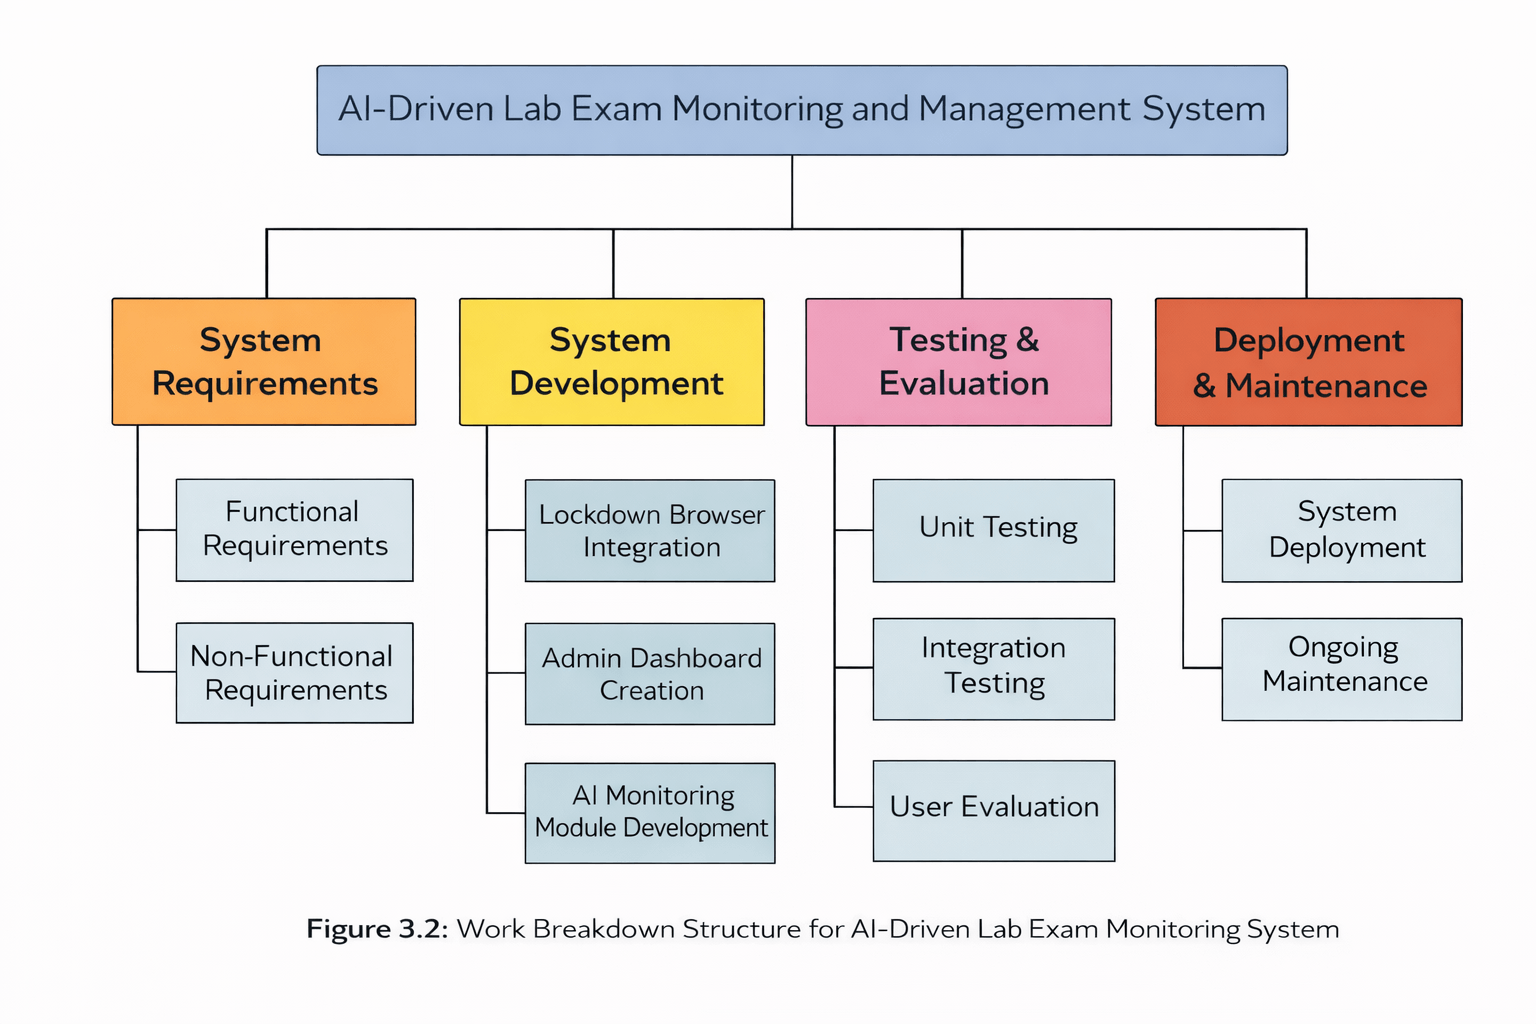
\includegraphics[width=0.95\linewidth]{Figures/work_breakdown_structure.png}
\caption{Work Breakdown Structure of the Proposed Project}
\label{fig:wbs}
\end{figure}

The WBS in Figure~\ref{fig:wbs} gives team members a clear picture of ownership. When a module appears in a sprint backlog, every team member knows exactly which WBS node it maps to. This prevents overlap and makes scope creep visible immediately \cite{spp1}.

\subsection{Critical Path Method}

The Critical Path Method (CPM) identifies which chain of activities determines the project's minimum completion time \cite{spp1}. Any delay along the critical path pushes the final deadline. Activities not on the critical path carry slack — they can slip slightly without affecting the overall schedule.

The project begins with Activity A (Gather Requirements, 1 week). From there, three parallel tracks run simultaneously. Track 1: Activity B (Lockdown Client Development, 3 weeks) followed by Activity E (AI Monitoring Module, 3 weeks). Track 2: Activity C (Admin Dashboard, 2 weeks), Activity D (Question Bank Module, 2 weeks), then Activity G (Unit Testing, 1 week). Track 3: Activity F (Student Exam Interface, 2 weeks). All three tracks converge at Activity H (Integration Testing, 1 week), followed by Activity I (System Deployment, 1 week). Figure~\ref{fig:criticalpath} shows the CPM network.

\begin{figure}[H]
\centering
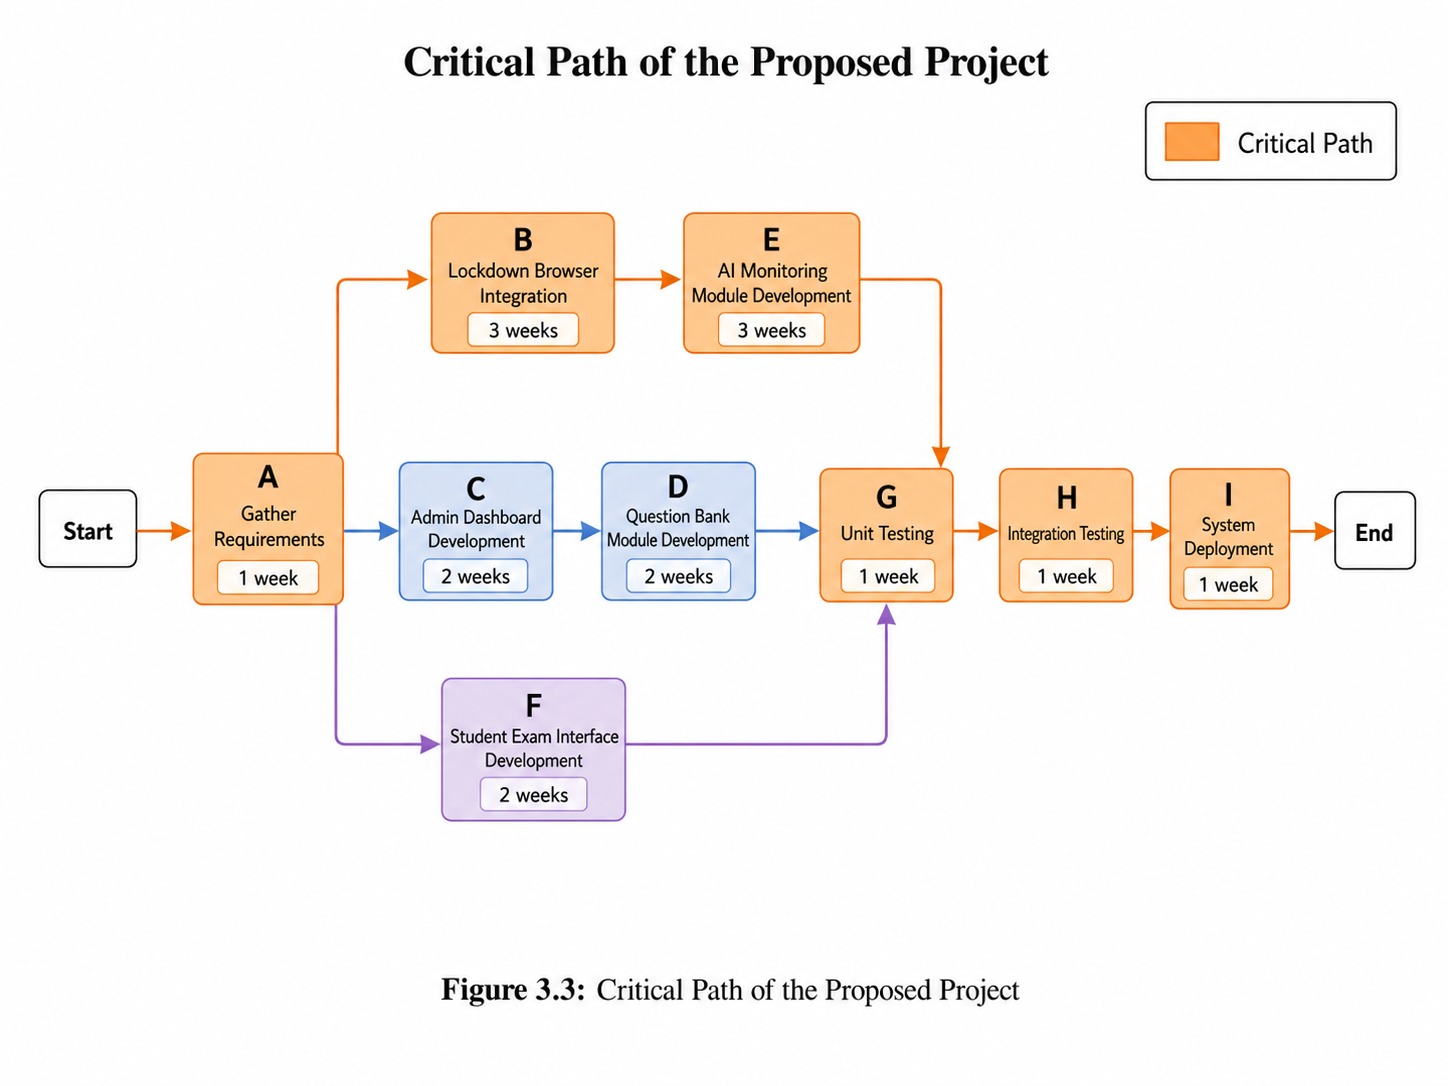
\includegraphics[width=0.95\linewidth]{Figures/critical_path.png}
\caption{Critical Path of the Proposed Project Activities}
\label{fig:criticalpath}
\end{figure}

The critical path runs A → B → E → H → I, totalling 9 weeks (1+3+3+1+1). Zero slack. Any delay to requirements gathering, the lockdown client, the AI monitoring module, integration testing, or deployment directly extends the delivery date. Track 2 carries 1 week of slack; Track 3 carries 4 weeks. These are the first areas to pull resources from if the critical path falls behind.

\subsubsection{Schedule Control and Review}

Schedule control uses sprint burn-down charts rather than passive calendar checks \cite{scrum1}. At the end of each sprint, the team compares planned story points against completed story points. If completion is below 80\% of the sprint target, a one-day recovery session is called before the next sprint begins. This keeps slippage visible early rather than hidden until the final integration sprint.
